%Linea Para poder completar automaticamente las citas con el Sublime
%No hace el documento, se puede borrar esta linea si no se usa el Sublime
%------------------------------------------------------------------------------
 \newcommand{\NoBiblioEQ}[1]{
 \ifthenelse{\equal{#1}{verdadero}}{}{\bibliography{Referencias/base_bibliografica}}
 \NoBiblioEQ{verdadero}}
 %----------------------------------------------------------------------------- 

%Formato (Nombre de capitulo largo o corto), nombre del capitulo y estilo de la
%Portada del Capitulo
%------------------------------------------------------------------------------

 %Formato en si, titulo en un solo renglon
 \FormatoCapituloDosLineas
 
 %Nombre y etiquete para referir
 \chapter{Propiedades de transporte\index{transporte} de los sensores}
 \label{chap:Electroquimica}

 %Para que no salga el numero de pagina en la portada del capitulo
 \thispagestyle{empty}
	
 %Resumen del Capitulo en Italica
 \noindent\textit{Aca va todo el desarrollo de la fisicoquimica de los mesospororos, fenomenos de  transporte, adsorcion, Langmuir\index{Langmuir}, propiedades de mediacion redox, catalisis, etc, etc.}

 %Indice de capitulo alineada al borde inferior de la pagina, nueva pagina
 \vfill
 \minitoc
 \newpage
 %-------------------------------------------------------------------------------

\section{Introducción}

	Una vez estudiados los distintos tratamientos de síntesis y realizada la fabricación de los sensores\index{sensor} se dedicará, en este capitulo, a estudiar las propiedades de los mismos para detectar y cuantificar una serie de sonda\index{sonda}s electroquímica\index{electroquimico}s\index{electroquimico} elegidas, precisamente, para poder evaluar distintos aspectos de transporte\index{transporte} a través de los sistemas nanoporosos. 
	Los sensores\index{sensor} están compuestos básicamente de una película delgada \index{película!delgada}de oro\index{oro} y una película delgada \index{película!delgada}nanoporosa\index{película!nanoporosa} de SiO$_2$. 

	La superficie\index{superficie} de las paredes dejan expuestos, hacia el interior de los poros, grupos silanoles los cuales pueden estar o no protonados.\cite{Brinker1990,Soler-Illia2011} 
			\begin{equation}
				\begin{aligned}
				\includegraphics[scale=0.75]{Esquemas/equilibriosilica.pdf}
				\label{eq:equilibriosilica}
				\end{aligned}
				\end{equation}

	La reacción \ref{eq:equilibriosilica} ejemplifica el equilibrio ácido-base que se establece en la superficie\index{superficie} de la sílice. El pKa del $\text{SiO}_2$ es menor a 4 y la mayoría de los autores coinciden en que el punto isoeléctrico\index{punto isoeléctrico} (PI) varía de $1$ a $4$ dependiendo de  las distintas forma alotrópicas del óxido de silicio\index{silicio!oxido de}, en particular para el SiO$_2$ sintetizado vía sol-gel\index{sol-gel} el $\text{PI}\approx 2$ \cite{Kosmulski2002,Kosmulski2014,Schwarz1984,Si-HanWu2013}.
	Wu\index{Wu} y colaboradores\cite{Si-HanWu2013} analizaron, por un lado, el estado de carga superficial de nanoparticula\index{nanoparticula}s\index{nanoparticula} de sílice mesoporosa\index{película!mesoporosa} y, por otro, la tasa de condensación\index{condensación}. El gráfico de la figura \ref{fig:silica_ph} muestra como varían las razones  $\text{SiO}^{-}/\text{SiOH}$ y $\text{SiOH}_2^{+}/\text{SiOH}$ en función del pH\index{pH}; se puede apreciar que solo por encima de $\text{pH}\geq7$ se obtiene una superficie\index{superficie} de carga negativa donde todos los silanoles reaccionaron, cediendo su $\text{H}^{+}$, para convertirse en iones silanoatos; mientras que para pH\index{pH} bajos ($\text{pH}\leq1$), la sílice se vuelve inestable antes de llegar a un estado de carga completamente positivo y, solo queda, parcialmente positiva. En el mismo trabajo\cite{Si-HanWu2013} también plantean que la tasa de condensación\index{condensación} decrece por encima de $\text{pH}\geq7.5$ debido a entra en una zona de inestabilidad donde el óxido se disuelve, catalizado por el medio básico.
			\begin{figure}[th!]
			\centering
 	       	\includegraphics[width=0.70\textwidth]{Graficos/Silica-PH-Stability.pdf}
	       		\caption[Tasa de condensación\index{condensación} y estado de carga superficial]{Tasa de condensación\index{condensación} y estado de carga superficial para nanoparticula\index{nanoparticula}s\index{nanoparticula} de sílice en función de pH\index{pH}. Gráfico extraído de \textit{Synthesis of mesoporous silica nanoparticles} Chem. Soc. Rev., 42(9):3862, 2013.\cite{Si-HanWu2013}}
	         	\label{fig:silica_ph}
	     		\end{figure}
			
	%Del equilibrio se desprende que al incrementar el pH\index{pH} por encima de $2$ la película presentará una carga neta negativa, y, consecuentemente al disminuir el pH\index{pH} por debajo de $2$ la película será neutra o levemente positiva. 
	De hecho, Iler\index{Iler}, en su libro \textit{<<The Chemistry of Silica>>}, explica que la tasa de disolución de la sílice en medio acuoso depende de muchos factores y, que además, salvando el tipo de sílice, el proceso de disolución requiere de un catalizador. Presenta un gráfico de la tasa de disolución en función del pH\index{pH} (figura \ref{fig:disolucion_ph}) y postula que la tasa de disolución depende de la forma alotropica de la sílice, mientras que para formas mas porosas como el SiO$_2$ amorfo la cinética de disolución es mas rápida, para otras como el cuarzo se hace mucho mas lenta; por último aclara que se trata de un proceso de despolimerización vía hidrólisis, y la solubilidad es la concentración de Si(OH)$_4$ cuando alcanza un estado estacionario en el equilibrio despolimerazación-polimerización.\cite{iler1979}. 

			\begin{figure}[th!]
			\centering
 	       	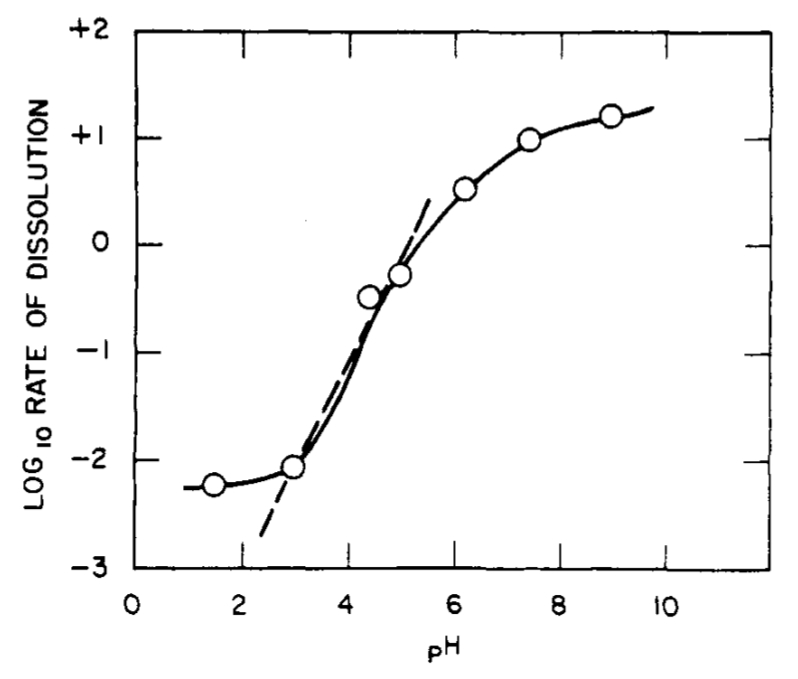
\includegraphics[width=0.70\textwidth]{Graficos/disolucion_ph.pdf}
	       		\caption[Tasa de disolución sílice en función del pH\index{pH}]{Tasa de disolución de la sílice en función de pH\index{pH}. Gráfico extraído de \textit{The chemistry of silica} Wiley 1ª edición, 1979.\cite{iler1979}}
	         	\label{fig:disolucion_ph}
	     		\end{figure}
	
	También propone un mecanismo en medio ácido\index{acido@ácido} catalizado por iones F$^-$, mientras que en medio básico\index{básico} el mecanismo es catalizado por iones OH$^-$, según el siguiente mecanismo:
			\begin{equation}
				\begin{aligned}
				\includegraphics[scale=0.60]{Esquemas/disolucionsilica.pdf}
				\label{eq:disolucionsilica}
				\end{aligned}
				\end{equation} 
	
	El mecanismo de \ref{eq:disolucionsilica} no está completamente consensuado en la literatura especializada, sin embargo todos los autores coinciden en que el óxido se vuelve inestable en cualquiera de sus forma alotrópicas a partir de un $\text{pH}\geq7$ y que, a partir de $\text{pH}\geq10$ el proceso de disolución se acelera considerablemente varios ordenes de magnitud.\cite{Kosmulski2002,Kosmulski2014,Schwarz1984,Si-HanWu2013,iler1979}

	%Dependencia de la constante de K con el PH.... poner aqui el grafico, ecuacion y grafico de Wu2013 donde propone estado de carga y donde se muestra que recien a PH=5 se llega a un estado de carga copmpeltamente negativo.
	
				
	%ca tengo que poner como es la reaccion del punto isoeléctrico\index{punto isoeléctrico} del Sio2 o del punto de carga zero... o del pka??? Y tambien tengo que poner los antecendente de calvo, calvo y el otro del 2005. Y tambien entonces que la diferencia es el Au\index{oro} miniaturizacion, etc, etc mayores velocidades... etc. 
	%No olvidarse de los ferrocenos a distintas velociades de barrido

\section{Transporte de sonda\index{sonda}s: exclusión, permeación\index{permeacion} y preconcentración}

	 Durante las próximas secciones se analizan e interpretan los resultados obtenidos al colocar soluciones con sonda\index{sonda}s electroquímica\index{electroquimico}s\index{electroquimico}, de diferente naturaleza, sobre los sensores. Al\index{aluminio} ser, la fabricación de los sensores, una parte estructural de este trabajo, cabe aclarar sobre que sistemas que se realizaron los resultados de los experimentos que se mostrarán de este capitulo; se utilizó, indistintamente, películas de Au\index{oro} sobre sustratos varios (silicio, vidrio, flexible), con diseño ya transferido o sin transferir. Salvo que se aclare lo contrario, se trabajó siempre sistemas con películas delgadas mesoporosas estructuradaras con Pluronic F127\index{Pluronic F127} y sintetizada con el método de alto vacio\index{alto@alto vacío} (consultar sección \ref{sec:trat-vacio}, pág. \pageref{sec:trat-vacio}); todas las medidas fueron normalizadas por el área geométrica, de forma de facilitar la comparación de resultados cuando se trata de sensores\index{sensor} con distinto diseño. Todas las medidas fueron llevadas a cabo a $\text{pH}\approx5,5$ en solución de KCl \SI{100}{\milli\Molar}, elegido con el propósito de mantener una fuerte carga neta negativa dentro de la películas, porque es un pH\index{pH} interesante para aplicaciones en aguas naturales, y a su vez, no está comprometida la disolución de la sílice.

	\subsection{Caso 1: sonda\index{sonda} de carga negativa}

	 El voltagrama de la figura \ref{fig:exclusion_vs_Au} muestra la respuesta de los sensores\index{sensor} cuando se colocan en una solución con una sonda\index{sonda} negativa. Como sonda\index{sonda} de carga negativa se utilizó ferro/ferriciunuro de potasio (\ferroferri, \SI{1}{\milli\Molar}) en proporciones equimolares. El voltagrama rojo corresponde a la respuesta en un electrodo de Au\index{electrodo!de Au}\index{oro} desnudo, mientras que la verde a un electrodo recubierto de \pdm.
	
			\begin{figure}[ht]
				\centering
		 	    \includegraphics[width=0.70\textwidth]{Graficos/ExclusionFcCN.pdf}
		        \caption[Exclusión electrostática]{Respuesta compartiva de un electrodo de Au\index{electrodo!de Au}\index{oro} recubierto con \pdmF\space y sin recubrir frente a una sonda\index{sonda} \ferroferri \SI{1}{\milli\Molar} en \SI{0.1}{\Molar} de KCl contra ESC.}
		        \label{fig:exclusion_vs_Au}
		      	\end{figure}
	
	 Al\index{aluminio} ser la sonda\index{sonda} de carga negativa, no es capaz de ingresar a la película (la cual está cargada negativamente), y, por lo tanto tampoco puede difundir hacia el electrodo, eso se refleja en el voltagrama donde no se observa ni reducción ni oxidación de la sonda\index{sonda}. La repulsión se debe a un efecto de exclusión electrostática. Este fenómeno de exclusión ya fue reportado por varios autores\cite{alberti2015,schmuhl2005,Andrieu-Brunsen2015,brunsen2011}. Al\index{aluminio} pH\index{pH} de trabajo, $\text{pH}=5,5$, los silinanoles están como \index{silanolato}s, como ya se explicó anteriormente, estableciendo una carga negativa en todo el espesor de la película.

	 Desde el punto del estudio de fenómenos de  transporte\index{transporte} esta sonda\index{sonda} no es especialmente útil, porque, como ya se demostró, no puede ingresar en la \pdm. Sin embargo, nos ofrece información importante sobre la integridad estructural de las películas delgadas, dicho de otro modo, al no obtener señal electroquímica\index{electroquimico} significa que, la sonda\index{sonda} no percola a través de la \pdm, que la \pdm\space se encuentra sin fisuras, agujeros o rajaduras y que recubre por completo el área del electrodo.

	 Por ende fue muy importante para corroborar (si no hay señal la película esta intacta, si hay señal esta el Au\index{oro} expuesto) el estado de las \pdm\space al finalizar experimentos donde se dudaba del estado de la película, de esta forma se utilizó esta sonda\index{sonda} a modo de <<experimento control>>, realizando una voltatametría cíclica\index{voltametria!cíclica} para comprobar que las películas no tuviera sitios de percolación.

	\subsection{Caso 2: sonda\index{sonda} de carga neutra}

		Al ser el ferroceno metanol\index{ferroceno metanol} (\fc) una molécula que, en su estado reducido, no presenta carga, es de esperar que no se vea afectada por la carga que presentan las paredes de los poros. En la figura \ref{fig:permeacion} se comparan los voltagramas resultantes de colocar una solución de ferroceno matanol sobre un electrodo de Au\index{electrodo!de Au}\index{oro} desnudo (voltagrama rojo) y uno recubierto con la \pdm.  Si bien el gráfico  requiere mas análisis, está claro que el ferroceno permea a través de la película nanoporosa, para dar una señal electroquímica\index{electroquimico}. En las próximas secciones se discutirá la forma, intensidad y otras variables de los voltagramas, y se analizarán experimentos complementarios, por ahora basta con haber demostrado que una sonda\index{sonda} neutra es sensible de permear a través de la \pdm\space para dar una señal electroquímica\index{electroquimico}.

		\begin{figure}[ht]
				\centering
		 	    \includegraphics[width=0.70\textwidth]{Graficos/FeOH-permeacion-1mM.pdf}
		        \caption[Permeación ferroceno metanol]{Respuesta compartiva de un electrodo de Au\index{electrodo!de Au}\index{oro} recubierto con \pdmF\space y sin recubrir frente a una sonda\index{sonda} \fc \SI{1}{\milli\Molar} en \SI{0.1}{\Molar} de KCl contra ESC.}
		        \label{fig:permeacion}
		      	\end{figure}
		%Ferroceno y todos los datos de permeacion. Calcinado vs Bajas Tcd 

	\subsection{Caso 3: sonda\index{sonda} de carga positiva}

		Para este caso se utilizó como sonda\index{sonda} cloruro de hexaminorutenio (III) (\aminorutenioCompleto, \ru), sonda\index{sonda} bien conocida por su reversibilidad entre los estados reducido y oxidado. Los primeros experimentos con está sonda\index{sonda} dan como resultados los voltagramas de la figuras \ref{fig:Ru10mM}. Al\index{aluminio}lí se muestra una serie continua de sucesivas voltametrías cíclicas y su evolución en el tiempo, desde el verde claro al verde oscuro. El cambio en la señal en función del tiempo se debe al ingreso el \ru\space a través de la matriz porosa, aumentando la intensidad de la señal conforme aumenta la concentración de la sonda\index{sonda} dentro de los poros. A su vez, también se observa un desplazamiento hacia un potencial mas reductor del pico anódico, esto se podría tomar como indicativo de un proceso de adsorción\index{adsorción} del \ru\space dentro de los poros. Dicha interacción se podría explicar como consecuencia de una interacción electrostática sonda\index{sonda}-pared, generando una señal <<mixta>> con dos contribuciones, la del \ru\space libre en solución o libre dentro de los poros y la del adsorbido en las paredes de la película mesoporosa, esto se manifiesta en los voltagramas de la figura \ref{fig:Ru10mM-resumen}.

		Con el objetivo de discriminar ambas contribuciones se realizó el siguiente experimento; una vez alcanza la intensidad de pico máxima se retira de la celda la solución con la sonda\index{sonda}, se reemplaza por solución que contiene únicamente electrolito soporte, de esta forma, de existir señal, solo tendría sentido si la misma proviene del \ru\space retenido en la película mesoporosa. El gráfico de la figura \ref{asd} muestra los resultados de dicho experimento, el mismo contiene tres voltagramas; el de color rojo corresponde a la respuesta de \ru\space en un electrodo de Au\index{electrodo!de Au}\index{oro} desnudo; la curva de color verde a la señal de una película <<cargada>> de \ru\space en solución de \ru; y la curva azul es el resultado de intercambiar la solución son la sonda\index{sonda} por solución con electrolito soportes unicamente. Esta última curva tiene la forma características que presentan las sonda\index{sonda}s adsorbidas, matrices con sitios redox\index{sitio redox\index{sitio redox}} <<anclados>>\cite{Ybarra2005} (como los que presentan los polímeros conductores) o los polímeros funcionalizados con compuestos electroactivos \cite{Rohlfing2005,Vila2015}, donde la separación de potencial entre los picos catodicos y anodicos es menor que \SI{60}{\milli\volt}, $\Delta E < \SI{60}{\milli\volt}$ 

			\begin{figure}[ht!]
				\begin{subfigure}[t]{0.495\textwidth}
				\includegraphics[width=1\textwidth]{Graficos/Ru10mM-ads-libre-flecha.pdf}
		        \caption{Ingreso de \ru\space \SI{10}{\milli\Molar} en una \pdmF.}
		        \label{fig:Ru10mM_ingreso}
		      	\end{subfigure}
		      	\begin{subfigure}[t]{0.495\textwidth}
				\includegraphics[width=1\textwidth]{Graficos/Ru10mM-Resumen.pdf}
		        \caption{Voltagramas donde se compara la señal en Au\index{oro} (\usebox{\rojo}), en una \pdmF\space(\usebox{\verde}) y en una \pdmF\space luego de retirar la solución de \ru (\usebox{\azul}).}
		        \label{fig:Ru10mM-resumen}
		      	\end{subfigure}
		      	\caption[Adsorción de sonda\index{sonda} positiva en \pdm]{Solución de \ru\space \SI{10}{\milli\Molar} en KCl \SI{100}{\milli\Molar} a $\text{pH}=5,5$. En a) se ve como aumenta la señal mientras la sonda\index{sonda} ingresa en la estructura porosa, en b) se muestra el adsorbido versus libre}
		      	\label{fig:primero-Ru10mM}
		      	\end{figure}


		Sin duda, bajo estas condiciones contorno, este es el caso mas interesante de los tres expuestos y el mas provechoso para estudiar propiedades físicas y químicas de los sistemas porosos. Los próximos apartados se centrarán en determinar variables de los sistemas mesoporosos y estudiar los fenómenos de transporte\index{transporte} que allí ocurren.

\section{Caso de estudio: \texorpdfstring{\ferroceno}{FeOH}}\label{sec:difusion}

	 Los resultados de la respuesta electroquimica del ferroceno metanol\index{ferroceno metanol} \linebreak (\ferroceno,\fc) en las \pdmF\space ya fueron presentados en la sección \ref{}, pág \pageref{key} del capitulo \ref{chap:Mesoporosos}. Sin embargo, en dicha sección, la discusión se centró en el análisis de la de películas delgadas mesoporosas y como cambia la accesibilidad\index{accesibilidad} en función de los distintos tratamientos de condensación\index{condensación} posdeposito.
	 En esta sección, se vuelven a discutir estos resultados, pero ahora en términos de fenómenos de transporte\index{transporte} y modelos válidos aplicables al calculo de coeficientes de difusión\index{difusión} del \fc\space en cada sistema.

	\subsection{En sistemas mesoporosos calcinados}

	 En los sistemas calcinados, aquellos en los que se eliminó el surfactante\index{surfactante} sometiendo las películas a \SI{350}{\celsius}, la red nanoporosa\index{película!nanoporosa} está mas accesible y mejor interconectada que aquellos que no fueron calcinados (ver capitulo \ref{chap:Mesoporosos}). Por lo tanto, se espera que la respuesta electroquímica\index{electroquimico} de la sonda\index{sonda} neutra, sea similar a la respuesta en un un electrodo de Au\index{electrodo!de Au}\index{oro} desnudo. En el voltagrama de la figura \ref{fig:fc_calcinado} se muestra que, efectivamente, se comporta de esta forma. Se colocó una solución de \fc\space \SI{1}{\milli\Molar} y se hicieron una serie de voltametrías a diferentes velocidades de barrido, con el propósito de calcular el coeficiente de difusión\index{difusión}. En el gráfico \ref{fig:difusion_calcinado}, donde se gráfico la intensidad de pico (i$_p$) en función de la velocidad de barrido\index{velocidad!de barrido} ($\nu$) se observa que $\text{i}_p \propto \nu^{1/2}$, lo que indica que se trata de un proceso controlado por difusión\index{difusión}. Ahora bien, esta difusión\index{difusión} tiene dos contribuciones, una de la sonda\index{sonda} en solución y otra de la sonda\index{sonda} dentro de los poros. 
		 \begin{equation}
					D=\frac{RT}{nF\nu}\left(\frac{\text{i}_p}{0.4463FAC}\right)^2
					\label{eq:dapp_bajaT}
			\end{equation}  
	 Se calculó, despejando de la ecuación de Randles-Sevcik\index{Randles-Sevcik} (ec. \ref{eq:dapp_bajaT}), el coeficiente de difusión\index{difusión} aparente ($D_{ap}$), el cual dió como valor $D_{app}$=\SI{6,1e-6}{\square\cm\per\second}, el cual es según la bibliografía un típico valor para moléculas en solución. \cite{koryta1993,Otal2006}

	 %Hacer un inset con un voltagrama a una velocidad de 50mV/s donde se aprecie bien la voltametria
			\begin{figure}[ht]
				\centering
		 	    \includegraphics[width=0.70\textwidth]{Graficos/FcOH-F127-Calcinado.pdf}
		        \caption[Voltagrama para \fc\space en \pdm\space calcinadas]{Voltagramas a diferentes velocidades de barrido para \fc\space \SI{1}{\milli\Molar} en solucion de KCl \SI{100}{\milli\Molar}. En el recuadro se amplia la VC para una velocidad de barrido\index{velocidad!de barrido} de \SI{20}{\milli\volt\per\second}.}
		        \label{fig:fc_calcinado}
		      	\end{figure}

		    \begin{figure}[ht]
				\centering
		 	    \includegraphics[width=0.70\textwidth]{Graficos/FcOH-F127-Calcinado-difusion.pdf}
		        \caption[i$_p$ en función de $\nu$ para \fc\space]{Intensidad e pico en función de la velocidad de barrido\index{velocidad!de barrido}. Se observa que $\text{i}_p$ es proporcional a $\nu ^{1/2}$, indicando que se trata de un transporte\index{transporte} controlado por difusión\index{difusión}.}
		        \label{fig:difusion_calcinado}
		      	\end{figure}
	      	
	\subsection{En sistemas mesoporoso sintetizados a baja temperatura}

		Se exponen en la figura \ref{fig:fcoh_bajaT} los voltagramas resultado de colocar \fc\space (1, 5 y \SI{10}{\milli\Molar}) utilizando como electrodo \pdmF\space condensada y extraída a bajas temperaturas (\SI{130}{\celsius}) por el método de alto vacio\index{alto@alto vacío}. 
			\begin{figure}[ht]
				\centering
		 	    \includegraphics[width=0.70\textwidth]{Graficos/FcOH-F127-BajaT.pdf}
		        \caption[Voltagrama para \fc\space en \pdm\space de baja temperatura]{Voltagramas de \fc\space 1, 5 y \SI{10}{\milli\Molar} en solución de KCl \SI{100}{\milli\Molar} tomados a una velocidad de barrido\index{velocidad!de barrido} de \SI{20}{\milli\volt\per\second}.}
		        \label{fig:fcoh_bajaT}
		      	\end{figure}
		
		En este caso se observa una respeta bien diferente que para el caso del calcinado, bajo las las mismas condiciones. Lo que sugieren estos resultados es que la difusión\index{difusión} a través de la película está disminuida respecto de los sistemas calcinados. Estos voltagramas son respuesta típica en sistemas donde se llega a un equilibrio, formando un gradiente de concentración a lo largo de la sección de la película y alcanzando una corriente límite $\text{i}_l$. 
		La forma de calcular el coeficiente de difusión\index{difusión} en estos sistemas es mediante la ecuación \ref{eq:de-ferroceno-bajaT} donde se calcula el coeficiente de difusión\index{difusión} $D$ a partir de $\text{i}_l$, de la diferencia de concentración entre las cercanías del electrodo ($C_{x=0}$) y el seno de la solución $C_s$, el aŕea ($A$) y el espesor de la película ($L$).

			\begin{equation}
					\text{i}_l = \frac{nFAD(C_{s}-C_{x=0})}{L}
					\label{eq:de-ferroceno-bajaT}
			\end{equation}
			  	

		Para una película de \SI{200}{nm} el $D$ resultó ser de \SI{2.5e-9}{\square\cm\per\second}, un valor esperado, ya que la difusión\index{difusión} se encuentra muy impedida en estos sistemas mas <<cerrados>>. El orden de magnitud de este valor es comparable con los reportados para polímeros electroactivos.\cite{Kolb1993}
			
\section{Caso de estudio: \texorpdfstring{\aminorutenioCompleto}{Ru(NH\index{amoniaco}3)CL3}}
	
	\subsection{Capacidad de preconcentración}

		Una vez demostrada la adsorción\index{adsorción} \ru\space de las \pdm, se llevaron a cabo una serie de experimentos adsorbiendo el analito partiendo de distintas concentraciones en solución, con el objetivo de determinar la capacidad de adsorción\index{adsorción}. La metodología es la misma que se aplicó en el experimento de la figura \ref{fig:Ru10mM-resumen}. Se utiliza un electrodo recubierto con la \pdmF\space, se miden repetidas voltametrías cíclicas hasta alcanzar el máximo de adsorción\index{adsorción}, esto ocurre cuando dos o más voltagramas consecutivos son equivalentes. Una vez alcanzado este punto, se retira la solución con la sonda\index{sonda} y se reemplaza con una nueva que sólo contienen electrolito soporte (KCl \SI{100}{\milli\Molar}). Se realiza entonces una nueva voltametría cíclica. Los resultados están expuestos en los voltagramas de la figura \ref{fig:preconcentraciones}, donde se ha llevado a cabo un barrido de concentraciones desde \SI{e-2}{\Molar} hasta \SI{e-5}{\Molar}. Cabe destacar que a concentraciones por debajo de \SI{60}{\micro\Molar} (con un área geométrica de \SI{1}{mm}) la sonda\index{sonda} ya no es detectada en un electrodo de Au\index{electrodo!de Au}\index{oro} desnudo, mientras que sobre una \pdm\space se preconcentra fuertemente.


				\begin{figure}[th]
			   	    \begin{subfigure}[t]{0.325\textwidth}
			        	\includegraphics[width=0.95\textwidth]{Graficos/Ru10mM.pdf}
			        	\vspace*{-0.40cm}\caption{\aminorutenio\space \SI{10}{\milli\Molar}.}
			         	\label{fig:Ru10mM}
			     		\end{subfigure}
			   	    \begin{subfigure}[t]{0.325\textwidth}
			        	\includegraphics[width=0.95\textwidth]{Graficos/Ru63mM.pdf}
			       		\vspace*{-0.40cm}\caption{\aminorutenio\space \SI{6}{\milli\Molar}.}
			         	\label{fig:Ru63mM}
			     		\end{subfigure}
		     		\begin{subfigure}[t]{0.325\textwidth}
			        	\includegraphics[width=0.95\textwidth]{Graficos/Ru315mM.pdf}
			       		\vspace*{-0.40cm}\caption{\aminorutenio\space \SI{3}{\milli\Molar}.}
			         	\label{fig:Ru315mM}
			     		\end{subfigure}
		     		\begin{subfigure}[t]{0.325\textwidth}
			        	\includegraphics[width=0.95\textwidth]{Graficos/Ru1575mM.pdf}
			       		\vspace*{-0.40cm}\caption{\aminorutenio\space \SI{1.5}{\milli\Molar}.}
			         	\label{fig:Ru1575M}
			     		\end{subfigure}
		 	   	   	\begin{subfigure}[t]{0.325\textwidth}
			        	\includegraphics[width=0.95\textwidth]{Graficos/Ru063mM.pdf}
			       		\vspace*{-0.40cm}\caption{\aminorutenio\space \SI{0.6}{\milli\Molar}.}
			         	\label{fig:Ru063mM}
			     		\end{subfigure}
		     		\begin{subfigure}[t]{0.325\textwidth}
			        	\includegraphics[width=0.95\textwidth]{Graficos/Ru0315mM.pdf}
			       		\vspace*{-0.40cm}\caption{\aminorutenio\space \SI{0.3}{\milli\Molar}.}
			         	\label{fig:Ru0315mM}
			     		\end{subfigure}
			     	 \begin{subfigure}[t]{0.325\textwidth}
			        	\includegraphics[width=0.95\textwidth]{Graficos/Ru0063mM.pdf}
			       		\vspace*{-0.40cm}\caption{\aminorutenio\space \SI{60}{\micro\Molar}.}
			         	\label{fig:Ru0063mM}
			     		\end{subfigure}
		     		\begin{subfigure}[t]{0.325\textwidth}
			        	\includegraphics[width=0.95\textwidth]{Graficos/Ru00315mM.pdf}
			       		\vspace*{-0.40cm}\caption{\aminorutenio\space \SI{30}{\micro\Molar}.}
			         	\label{fig:Ru00315mM}
			     		\end{subfigure}
		     		\begin{subfigure}[t]{0.325\textwidth}
			        	\includegraphics[width=0.95\textwidth]{Graficos/Ru001575mM.pdf}
			       		\vspace*{-0.40cm}\caption{\aminorutenio\space \SI{15}{\micro\Molar}.}
			         	\label{fig:Ru001575mM}
			     		\end{subfigure}	
		 	   	   	\caption[Preconcentración de \aminorutenio]{Adsorción de \ru\space en \pdm\space a diferentes concentraciones de la sonda\index{sonda}. Los voltagramas grises (\usebox{\gris}) indican el ingreso de la sonda\index{sonda} en la red nanoporosa, los azules (\usebox{\azul}) corresponden a la sonda\index{sonda} adsorbida en solución con electrolito soporte únicamente y los voltagramas rojos (\usebox{\rojo}) son la respuesta en electrodos de Au\index{electrodo!de Au} desnudo. Todos los voltagramas fueron medidos a \SI{50}{\milli\volt\per\second} en solución de KCl \SI{100}{\milli\Molar}.}
		     		\label{fig:preconcentraciones}
		     	   	\end{figure} 	

		Se puede calcular la concentración dentro de la \pdm, es decir la concentración adsorbida de \ru\space, de acuerdo a la ecuación \ref{eq:concentracion}, donde $C$ es la concentración, $Q$ es la carga eléctrica, $F$ la constante de Faraday\index{Faraday}, $A$ el área geométrica y $d$ el espesor de la nanopelícula la cual fue medida previamente por las técnicas explicadas en el capitulo \ref{chap:Materiales}, ya sea EPA o FIB\index{FIB}.

			\begin{equation}
					C=\frac{Q}{FAd}
					\label{eq:concentracion}
			\end{equation}

		La $Q$ es igual a la integral de la corriente en el tiempo. Se puede desarrollar dicha igualdad \ref{eq:carga} y resolver como la integral entre dos valores de potencial para una velocidad de barrido\index{velocidad!de barrido} constante (\SI{50}{\milli\volt\per\second}) para los experimentos de la figura \ref{fig:preconcentraciones}). Por lo tanto, para cada voltagrama de la figura \ref{fig:preconcentraciones}, se puede extraer el valor de $Q$, tanto para la corriente anódica como para la catódica.
		
			\begin{equation}
					Q=\int i\,dt = \int i\, \frac{dt}{dE} dE = \int i\,\frac{1}{v}dE=\frac{1}{v}\int_{E_{i}}^{E_{f}} i\,dE
					\label{eq:carga}
			\end{equation}

		Una vez obtenidas estos valores se gráfica la isoterma\index{isoterma} de adsorción\index{adsorción} a T=\SI{25}{\celsius} (figura \ref{fig:langmuir}. De esta curva se obtiene una relación analítica entre la concentración de \ru\space dentro de la \pdm\space y la concentración de \ru{\ru}\space que colocamos inicialmente. La isoterma\index{isoterma} resultante se corresponde con una <<isoterma de Langmuir\index{Langmuir}>> donde la cantidad adsorbida aumenta hasta alcanzar un valor límite, correspondiente a recubrir de la superficie\index{superficie} de la \pdm por una monocapa, debido a la quimisorción del \ru.\cite{langmuir1918}

			\begin{figure}[ht]
					\centering
			 	    \includegraphics[width=0.70\textwidth]{Graficos/langmuir.pdf}
			        \caption[Isoterma de Langmuir\index{Langmuir}]{Isoterma de Langmuir\index{Langmuir} a T=\SI{25}{\celsius}donde se gráfica la concentración de \aminorutenio\space adsorbido en función de la concentración en solución colocada inicialmente.}
			        \label{fig:langmuir}
			      	\end{figure} 	
	
		Según la ecuación de Langmuir\index{Langmuir} para este tipo de isortermas, el grado de recubrimiento ($\theta$) esta determinado por la concentración en solución ($C_{sol}$) y la constante de equilibrio de la adsorción\index{adsorción}/desorción ($K$). Del ajuste de la curva podemos extraer $K$ y, la cual para nuestro sistema es de $K=$\SI{9e3}{\Molar^{-1}}. También podemos calcular la concentración de \ru\space dentro de la película delgada \index{película!delgada}en condiciones de saturación, la cual es de $C=$\SI{1.1}{\Molar} para un espesor de película de \SI{200}{nm}.

			\begin{equation}
					\theta = \frac{KC_{sol}}{KC_{sol}+1}
					\label{eq:langmuir}
			\end{equation}
		Si bien ya se han reportado la adsorción\index{adsorción} de sonda\index{sonda}s positivas en sistemas similares (por ejemplo en el trabajo de Etienne\index{Etienne} y col. \cite{Etienne2007}, donde adsorbe $\text{Ru}(bpy)_3^{2+}$ en una película de sílice mesoporosa\index{película!mesoporosa} sobre ITO a $\text{pH}=4.1$) no se ha reportado, hasta la fecha, cálculos de concentraciones dentro de las películas delgadas.

	\subsection{Mecanismo de transporte\index{transporte} de carga}

	 Como ya se demostró anteriormente, el sistema adsorbe la sonda\index{sonda} sobre las paredes de la película delgada \index{película!delgada}formando una monocapa. Se genera entonces, un par iónico\index{iónico} entre el \ru, de carga positiva (+2 o +3 dependiendo del estado de oxidación), y los \index{silanolato}s de las paredes del mesoporoso, cuya carga es negativa. Los sitios redox\index{sitio redox\index{sitio redox}} ($\phi^{e}$) están parcial o totalmente inmovilizados, sugiriendo que el mecanismo de transferencia de carga es el que se produce a través de saltos electrónicos entre los sitios redox\index{sitio redox\index{sitio redox}}, o como se lo conoce mas comúnmente en ingles, \textit{electron hopping}\index{electron hopping}. %Una cita por aca. 
	 Si se supone nanoporos esféricos, monodispersos y distribuidos uniformemente en la película (consultar capítulo \ref{chap:Mesoporosos}), se puede estimar la cantidad \ru\space por poro. Para ello se multiplica la concentración de \ru\space adsorbido ($C$), por la fracción porosa ($F_p$), por el volumen de un sólo poro\index{poro} ($V_{poro}$ y por el número de Avogrado\index{Avogadro} ($N_{A}$) para calcular el numero de moléculas. Y, a su vez, como se encuentran adsorbidos, se puede dividir por la superficie\index{superficie} del poro\index{poro} ($S_{poro}$) de forma de obtener el numero de sitios redox\index{sitio redox\index{sitio redox}} por unidad de volumen, o, tomando la raíz cuadrada de la inversa, la distancia promedio entre dos sitios redox\index{sitio redox\index{sitio redox}} ($d_{\phi^{e}}$), según la ecuación \ref{eq:distancia_redox}. 
	 	\begin{equation}
					d_{\phi^{e}}=2\sqrt{\frac{S_{poro}}{\pi\, V_{poro}\, N_A\, C\, F_p}}
					\label{eq:distancia_redox}
			\end{equation}
	 Teniendo en cuenta una concentración de saturación de \SI{1}{\Molar} en una película de \SI{200}{nm} con una porosidad\index{porosidad} $F_p=35\%$, la distancia promedio entre sitios redox\index{sitio redox\index{sitio redox}} resulta de $d_{\phi^{e}}=$\SI{1.25}{nm}. Esta estimación (aún con los suposiciones de poros esféricos e idénticos) es compatible con el modelo de \textit{eletron hopping} propuestos y con la concentración calculada. Un valor muy grande, p. ej. $d_{\phi^{e}}>15\, \text{nm}$ seria un indicador de que, o bien la película no esta saturada o bien los sitios redox\index{sitio redox\index{sitio redox}} están muy lejos para permitir el salto entre sitios, mientas que un valor de $d_{\phi^{e}}$ muy pequeño, seria comparable con el radio de la sonda\index{sonda} y se solaparían los sitios redox\index{sitio redox\index{sitio redox}} (para $d_{\phi^{e}} < r_{\phi^{e}}$). 
	 		\begin{figure}[ht!]
					\centering
			 	    \includegraphics[width=0.60\textwidth]{Esquemas/sitios_redox.pdf}
			        \caption[Mecanismo de transferencia de electrones]{Diagrama en el cual se ejemplifica el mecanismo de trasnferencia y transporte\index{transporte} de carga mediante saltos electrónicos o \textit{electron hopping}\index{electron hopping}.}
			        \label{fig:sitios_redox}
			      	\end{figure} 	
	
	 En el esquema de la figura \ref{fig:sitios_redox} se ejemplifica el mecanismo propuesto y se puede, entonces, calcular el coeficiente de difusión\index{difusión} $D_e$ para la transferencia de electrones. Se abarcó el calculo de este parámetro desde dos enfoques diferentes, uno utilizando la técnica de voltametría de corriente alterna\index{voltametría!de corriente alterna} (VCA) y otra utilizando voltametrías cíclicas (CV) a distintas velocidades de barrido. Los detalles experimentales para ambas técnicas fueron explicados en la sección \ref{sec:medidas_eq}, pág. \pageref{sec:medidas_eq}.
	  
	 \subsubsection*{Calculo de $D_e$ mediante VC}	
	 
	   	 Para calcular el $D_e$ se tomaron VCs de una películas mesoporosas saturadas con \ru\space a distintas velocidades de barrido, desde \SI{50}{\milli\volt\per\second} a \SI{50}{\volt\per\second}. Luego se graficó el desplazamiento del\index{potencial!de pico} por un lado y la intensidad de pico por otro, ambas variables en función de la velocidades de barrido (gráficos \ref{fig:corrimiento-potenciales} y \ref{fig:ip-vel} respectivamente). De acuerdo al trabajo de Tagliazucchi\index{Tagliazucchi} y Calvo\index{Calvo}\cite{Tagliazucchi2010a} (donde calcula el coeficiente de difusión\index{difusión} para un complejo de osmio adsorbido en un polímero), es posible, a partir del tiempo de difusión\index{difusión} característico (ec. \ref{eq:tao_caracteristico}),\hfill
	   		\begin{equation}
					\tau_{\scriptscriptstyle{D}}=\frac{d^2}{2\ D_e}
					\label{eq:tao_caracteristico}
			 \end{equation}
	   	 determinar la velocidad de barrido\index{velocidad!de barrido} característica (ec. \ref{eq:v_caracteristica}) para la cual la capa de difusión\index{difusión} alcanza la interfase de la solución.  
 		   	 \begin{equation}
					\nu_{\scriptscriptstyle{D}}=\frac{RT}{\tau_{\scriptscriptstyle{D}}F}
					\label{eq:v_caracteristica}
			 \end{equation}
		 Es en esta velocidad característica donde la respuesta del potencial cambia entonces de un comportamiento de capa delgada \index{película!delgada}a un comportamiento controlado por difusión\index{difusión}. La figura \ref{fig:corrimiento-potenciales} muestran con flechas rojas la velocidad característica donde aparentemente la transferencia de carga es mas rápido que el transporte\index{transporte} de carga, sin embargo el procesos de transferencia de carga enmascara la separación de picos y, por lo tanto, es difícil establecer $\nu_{\scriptscriptstyle{D}}$ de este gráfico.
			 \begin{figure}[ht]
					\centering
			 	    \includegraphics[width=0.70\textwidth]{Graficos/MARIO-Ru1mM-Potenciales.pdf}
			        \caption[Desplazamiento de potenciales]{Desplazamiento de los potenciales en función de la velocidad de barrido\index{velocidad!de barrido}, las flechas rojas indican la velocidad característica para el cambio de régimen, de capa delgada \index{película!delgada}a control difusional.}
			        \label{fig:corrimiento-potenciales}
			      	\end{figure}
         La figura \ref{fig:ip-vel} muestra la corriente de pico en función de la velocidad de barrido\index{velocidad!de barrido}. Para una velocidad $\nu \approx \nu_{\scriptscriptstyle{D}}$ se observa una transición de régimen en capa delgada \index{película!delgada}($\text{i}_{p} \propto \nu$) a régimen controlado por difusión\index{difusión} ($\text{i}_{p} \propto \nu^{1/2}$).	Este gráfico permite estimar con menor interferencia el cambio de regimen y por lo tanto la $\nu_{\scriptscriptstyle{D}}$, la cual se ha identificado en el gráfico con flechas rojas. En la figura \ref{fig:ip-vel2} donde se graficó log{i$_p$} vs log{$\nu$} se hace evidente el cambio de régimen de capa delgada \index{película!delgada}(pendiente=1) a controlado por difusión\index{difusión} (pendiente=0.5).

		 Una vez que obtenemos el valor de  $\nu_{\scriptscriptstyle{D}}$ se combinan las ecuaciones \ref{eq:tao_caracteristico} y \ref{eq:v_caracteristica} para obtener finalmente el valor del coeficiente de difusión\index{difusión} de saltos electrónicos entre sitios redox\index{sitio redox\index{sitio redox}},  $D_e$ (ecuación \ref{eq:dh}. Para nuestro sistema resultó\hfill\linebreak$D_e=$\SI{1.6e-9}{\square\cm\per\second}.  
			\begin{equation}
					D_e= \frac{d^2\nu_{\scriptscriptstyle{D}}F}{2RT}
					\label{eq:dh}
			\end{equation}
            \begin{figure}[ht]
			  \begin{subfigure}[t]{0.495\textwidth}
			  \includegraphics[width=1\textwidth]{Graficos/MARIO-Ru1mM-ip-vel.pdf}
			  \caption{Intensidad de pico  en función de la velocidad de barrido\index{velocidad!de barrido}, las flechas rojas indican la velocidad característica para el cambio de régimen.}
			  \label{fig:ip-vel}
		  	 \end{subfigure}	
			 \begin{subfigure}[t]{0.495\textwidth}
			  \includegraphics[width=1\textwidth]{Graficos/MARIO-Ru1mM-Max-Min.pdf}
			  \caption{Log(i$p$) vs log($\nu$) para determinar el cambio de régimen.}
			  \label{fig:logj-logv}
		  	 \end{subfigure}
			  \caption[Calculo de velocidad de barrido\index{velocidad!de barrido} característica]{Gráficos para determinar $\nu_{\scriptscriptstyle{D}}$, en a) marcada con flechas rojas donde es mas sencillo de determinar debido a la independencia del potencial; en b) mediante el cambio en la pendiente de  régimen en capa delgada \index{película!delgada}($\text{i}_{p} \propto \nu$) a régimen controlado por difusión\index{difusión} ($\text{i}_{p} \propto \nu^{1/2}$).}
			  \label{fig:ip-vel2}
			  \end{figure}
	 
	 \subsubsection*{Calculo de $D_e$ mediante AVC}

    	 El segundo enfoque que se utilizó para calcular $D_e$ fue mediante el uso de la técnica de voltametría de corriente alterna\index{voltametría!de corriente alterna} (ACV). Esta técnica muy útil para el estudio de factores cinéticos en sistemas reversibles, permite fácilmente, para pequeñas perturbaciones, discriminar la componente de corriente continua de la de corriente alterna en función del potencial aplicado. Los voltagramas de la figura \ref{fig:acv} muestran la respuesta de una \pdmF\space cargada con \ru. Se aplicó una una perturbación de \SI{10}{\milli\volt} a una frecuencia de 1 y \SI{2}{\hertz}.

	 			\begin{figure}[ht]
					\centering
			 	    \includegraphics[width=0.70\textwidth]{Graficos/ACV-1-2Hz.pdf}
			        \caption[Voltametrías de corriente alterna]{Voltametría de corriente alterna para una película satura con \ru. Se aplicó una perturbación de 10mV y una frecuencia de 1 y \SI{2}{\hertz} en solución de KCl \SI{100}{\milli\Molar} usando como referencia ESC.}
			        \label{fig:acv}
			      	\end{figure}

    	 El desarrollo de descomponer y combinar las ecuaciones para las componentes de corriente alterna y directa en función de campo eléctrico, deriva en una ecuación que nos permite calcular el coeficiente de difusión\index{difusión} \cite{Wi2000}, el cual dió como resultado $D_e$=\SI{4.5e-9}{\square\cm\per\second}. 
    	 	
    	 		\begin{equation}
					D_e=\sqrt{\frac{i_p\ 4RT}{n^2 F^2 A C \Delta E \omega ^{1/2}}}
					\label{eq:acv}
				 \end{equation}

		Resulta interesante remarcar las diferencias de ambos métodos. El primero se basa en calcular la velocidad de barrido\index{velocidad!de barrido} característica para el espesor de una película delgada. El segundo utiliza el dato de la concentración de adsorbato para estimar el coeficiente de difusión\index{difusión} mediante la técnica de ACV. Ambos métodos, estiman el valor de $D_e$ desde diferentes aproximaciones, dando un valor de $D_e$ comparable y dentro del mismo orden de magnitud (\SI{e-9}{\square\cm\per\second}) validando el modelo que se propuso para el sistema estudiado.
			
	\subsection{Simulaciones por elementos finitos}	

		A partir de la experiencia acumulada, y en base al modelo propuesto sobre el trasporte de carga para estos sistemas preconcentradores, se planteó la posibilidad de utilizarlos como mediadores electroquímico\index{electroquimico}s\index{electroquimico}. 
    	La mediación\index{mediacion} en sistemas análogos, basados en polímeros con complejos electroactivos, es bien conocida.\cite{Kolb1993,Ybarra2005}. Por lo tanto, para determinar si son sistemas con la capacidad de transportar la carga de una sonda\index{sonda} electroquímica\index{electroquimico} (ya sea neutra, positiva o negativa) desde la interfase mesoporoso-solución hasta el electrodo, se diseño un experimento de mediación\index{mediacion} electroquímica\index{electroquimico}. El mismo consintió en cargar una \pdmF\space completamente de \ru, retirar la solución y colocar una solución con \fc en electrolito soporte, KCl \SI{100}{\milli\Molar}. El voltagrama de la figura \ref{fig:mediacion} muestra la respuesta que se obtuvo de este experimento (\usebox{\verde}) y se comparada, en el mismo gráfico, con un voltagrama de \fc\space en una \pdmF\space no cargada (\usebox{\azul}) y en un electrodo de Au\index{electrodo!de Au}\index{oro} desnudo (\usebox{\rojo}).  

        	\begin{figure}[ht]	
					\centering
			 	    \includegraphics[width=0.70\textwidth]{Graficos/mediacion.pdf}
			        \caption[Voltagrama de \ru\space y \fc.]{Mediciones electroquimicas de \fc\space \SI{5}{\milli\Molar} en solución de KCl \SI{100}{\milli\Molar} sobre un electrodo de Au\index{electrodo!de Au}\index{oro} desnudo (\usebox{\rojo}), sobre una \pdmF\space (\usebox{\azul}) y sobre una \pdmF\space con \ru\space adsorbido (\usebox{\verde}.}
			        \label{fig:mediacion}
			      	\end{figure}

		Allí se observa que la señal del \fc\space es de una intensidad comparable con la que la que se obtiene en un electrodo de Au\index{electrodo!de Au}\index{oro} desnudo. Se sugieren a partir de estos resultados dos hipótesis. Que la señal del \fc\space se debe a una mediación\index{mediacion} electroquímica\index{electroquimico} entre el rutenio y el electrodo, o bien que  el \fc\space está permeando a través de la película por algún cambio debido a la adsorción\index{adsorción} del \ru\space en la película. Cabe destacar que la señal del \fc\space en la película cargada de \ru\space es mucho mas intensa que la que corresponde a colocar \fc\space en una \pdmF\space sin \ru.

		Para poder discriminar e interpretar cual es el proceso que está dando origen a la señal, se recurrió a experimentos de simulación. Se trabajo en conjunto con el Dr. Mario Tagliazucchi\index{Tagliazucchi} del Instituto de Química Física de los Materiales, Medio Ambiente y Energía (INQUIMAE\index{INQUIMAE}) haciendo simulaciones por elementos finitos.

		Se utilizó un modelo en el que se tienen en cuenta un electrodo recubierto con una película delgada \index{película!delgada}\SI{200}{nm} saturada de  \aminorutenio en una concentración de \SI{1}{\Molar}. Para una descripción detallada de los parámetros utilizados se pueden consultar en la sección \ref{simulacion}, \pageref{simulacion}. 

		La primera simulación\index{simulacion} (figura \ref{fig:sim_mediacion}) tiene en cuenta dos sonda\index{sonda}s, una adsorbida y otra libre en solución (en los caso experimentales presentados \ru\space y \fc\space respectivamente), y se varía la diferencia del potencial de reducción estándar entre ambas sonda\index{sonda}s, $\Delta E$. El objetivo de esta simulación\index{simulacion} es establecer alguna valor limite de $\Delta E$ a partir del cual la mediación\index{mediacion} es posible. Debe existir un mínimo solapamiento entre los potenciales de reducción/oxidación de ambas especies, de modo tal que una fracción de la población de los sitios redox\index{sitio redox\index{sitio redox}} anclados en la película puedan transferir carga a la sonda\index{sonda} en la solución en la interface\index{interface} película-solución.

			\begin{figure}[ht]
					\centering
			 	    \includegraphics[width=0.70\textwidth]{Graficos/FcOH-Simulacion-deltaE.pdf}
			        \caption[Simulación EQ de mediación\index{mediacion} redox]{Simulación por elementos finitos del voltagrama para la mediación\index{mediacion} entre una sonda\index{sonda} en solución y una \pdmF\space con \ru\space \SI{1}{\milli\Molar} en función de la diferencia de potencial estándar para cada una de las sonda\index{sonda}s.}
			        \label{fig:sim_mediacion}
			      	\end{figure}

		Del análisis de la simulación\index{simulacion} se desprende que la mediación\index{mediacion} electroquímica\index{electroquimico} es posible. Sin embargo para $\Delta E >$\SI{300}{\milli\volt} la intensidad de la sonda\index{sonda} en solución disminuye sensiblemente y para \SI{400}{\milli\volt} es prácticamente nula. La separación de potenciales estándar del \aminorutenio\space y del \fc\space es de aproximadamente \SI{400}{\milli\volt} tomada sobre medidas en soluciones independiente, para cada sonda\index{sonda}, en electrodos de Au\index{electrodo!de Au} (consultar sección \ref{sec:respuesta_sondas_au}, \pageref{sec:respuesta_sondas_au}). Por la tanto, es de esperar que la señal observada para el \fc\space en la figura \ref{fig:mediacion} se trate de un proceso de permeación.

		Se realizaron dos nuevas simulaciones, ahora permitiendo que simultáneamente ocurran los procesos de mediación\index{mediacion} y permeación. Los parámetros variables fueron el coeficiente de difusión\index{difusión} del \fc\space dentro de la película, $D_{Fc}$ y la constante para la reacción de mediación\index{mediacion} redox, $k$. En el gráfico \ref{fig:sim_med_k0}, la mediación\index{mediacion} no es posible por imposición de la simulación, donde $k=0$. Al\index{aluminio}lí se observa que la permeación\index{permeacion} ocurre para $D_{Fc}\lesssim$\SI{e-10}{\square\cm\per\second} y para $D_{Fc}\gtrsim$\SI{e-6}{\square\cm\per\second} llega a un valor limite y la respuesta se mantiene constante.

		En el caso de hacer simulaciones que permitan la mediación\index{mediacion} redox, con un valor de $k=$\SI{1000}{\per\Molar\per\second}, se pone de manifiesto que la permeacion es el proceso dominante para valores de $D_{Fc}\gtrsim$\SI{e-6}{\per\Molar\per\second} y que, si bien es pobre, la mediación\index{mediacion} redox se dá para valores de $D_{Fc}\lesssim$\SI{e-8}{\per\Molar\per\second}.

			\begin{figure}[ht]
				\begin{subfigure}[t]{0.495\textwidth}
					\centering
			 	    \includegraphics[width=1\textwidth]{Graficos/FcOH-Simulacion-K0DFcOH.pdf}
			        \caption{Simulacion de mediación\index{mediacion} y permeacion con $k=0$.}
			        \label{fig:sim_med_k0}
			      	\end{subfigure}
				\begin{subfigure}[t]{0.495\textwidth}
					\centering
			 	    \includegraphics[width=1\textwidth]{Graficos/FcOH-Simulacion-K1000DFcOH.pdf}
			        \caption{Simulación de mediación\index{mediacion} y permeación\index{permeacion} con $k=1000$.}
			        \label{fig:sim_med_1000}
			      	\end{subfigure}
			      	\caption[Simulación EQ de mediación/permeación]{Simulaciones de permeación\index{permeacion} y mediación\index{mediacion} redox para una \pdm\space de \SI{200}{nm} de espesor cargada de \ru\space \SI{1}{\Molar}. Se simularon para dos constantes de mediación, $k=0$ y $k=1000$ \si{\per\Molar\per\second} variando el coeficiente de difusión\index{difusión} del \fc\space dentro las películas.}
			      	\label{fig:sim_med_perm}
			      	\end{figure}
			      	
		Comparando los experimentos simulados con los experimentos realizados en el laboratorio (figura \ref{fig:comp_sim_exp}), se puede interpretar cual es el fenómeno de transporte\index{transporte} de carga/masa dominante en los sistemas estudiados. 

				\begin{figure}[ht]
					\centering
			 	    \includegraphics[width=0.70\textwidth]{Graficos/Comparacion-exp-simulado.pdf}
			        \caption[Simulación EQ comparadas con datos experimentales]{Comparación entre resultados experimentales y de simulación. Los parámetros de la simulación\index{simulacion} fueron $k=$\SI{1000}{\per\Molar\per\second}, $D_{Fc}=$ \SI{e-6}{\square\cm\per\second} con \fc\space \SI{5}{\milli\Molar} en un \pdm\space con \ru\space adsorbido \SI{1}{\Molar}. El experimento de laboratorio fue realizado con las mismas concentraciones para ambas sonda\index{sonda}s.}
			        \label{fig:comp_sim_exp}
			      	\end{figure}
		
		En la sección \ref{sec:difusion} se calculo el coeficiente de difusión\index{difusión} del \fc\space utilizando los sistemas fabricados a bajas temperatura por el método de alto vacio\index{alto@alto vacío}, el cual resulto ser $D_{Fc}=$\SI{2.5e-9}{\per\Molar\per\second}. Bajo estas condiciones, deberíamos observar en los resultados experimentales, de acuerdo a las simulaciones, ambos fenómenos, mediación\index{mediacion} redox y permeación.

		Resulta evidente que sólo el fenómeno de permeación\index{permeacion} es el dominante, sugiriendo un cambio en el coeficiente de difusion del \fc, de $D_{Fc}=$\SI{2.5e-9}{\per\Molar\per\second} a, por lo menos, $D_{Fc}\!=$\SI{e-6}{\per\Molar\per\second}, el cual se aproxima al calculado para sistemas calcinados,  $D_{Fc}=$\SI{6.1e-6}{\per\Molar\per\second} (ver sección \ref{sec:difusion}, pág. \pageref{sec:difusion}). La interpretación de estos resultados es que los sistemas porosos condensados y extraídos a baja tempratura van cambiando su estructura a medida que el \ru\space se adsorbe en su superficie\index{superficie}, permitiendo, luego que el \fc\space difunda mas libremente hacia el electrodo, asemejándose a los sistemas calcinados. Como veremos en la próxima sección esto responde a un proceso de disolución de la sílice catalizado por la adsorción\index{adsorción} de \aminorutenio.

	\subsection{Disolución y ventana de trabajo}

		Como ya se ha demostrado, que al poner en contacto una solución de \ru\space sobre una \pdmF\space, la película se va cargando hasta alcanzar la saturación. Es de esperar la carga dentro de la película se mantenga constante y que, a partir del voltagrama de máxima adsorción\index{adsorción} las sucesivas voltametrías sean equivalentes.

		Sin embargo, no es así, y al ciclar constantemente el sistema se obtienen los voltagramas de la figura \ref{fig:diso_ru1mM}, experimento donde se adsorbió \ru\space \SI{1}{\milli\Molar}. Se observa que el mesoporoso se va va cargando conforme aumenta el numero de ciclos, y adsorbiendo cada mas \ru\space, hasta llegar a un máximo de adsorción\index{adsorción}, indicado por la curva azul. Si se continua ciclando el sistema el mismo evoluciona hasta la curva roja, la cual coincide con un voltagrama para \ru\space medido sobre un electrodo de Au\index{electrodo!de Au}\index{oro} desnudo. Esto indica que las \pdm\space se disuelven luego de hacer algunos ciclos de VC.

		Si bien estamos en a un pH\index{pH} ($5.5$) donde la disolución de las \pdm\space debería ser mínima o nula, las mismas parecen disolverse con bastante facilidad, ya sean \pdm\space calcinadas o sin calcinar. De estos resultados surgió la disyuntiva de que, si la disolución se debe al pH\index{pH}, a la sonda\index{sonda} o al potencial aplicado. Se han aislado estas variables dejando sumergidas las \pdm en solución con electrolito soporte (KCl \SI{100}{\milli\Molar}), con y sin \ru\space durante varios días y no se ha observado disolución alguna de las \pdm. Tampoco se ha observado disolución cuando se utilizan sonda\index{sonda}s neutras o negativas, como \fc, \HQ o \fcn. 

		Solo se disuelven cuando se adsorbe \ru\space fenomeno de sqeeling, debido al ingreso e ingreso de contraiones para balancear la carga, ....

		% Si bien se ha demostrado la adsorción\index{adsorción} del \aminorutenio\space en las \pdm, se deben establecer las condiciones de contorno para las cuales estos resultados tienen validez. Ya que, al ciclar el sistema (tal como se explico en el apartado anterior) sucesivamente la \pdm se disuelven. Este comportamiento, es, cuanto menos llamativo. Al\index{aluminio} pH\index{pH} de trabajo 
	 % 	se basaron en trabajos que utilizan, o esta misma sonda\index{sonda}\cite{} o sonda\index{sonda}s de rutenio bipiridina. Losresultados fue el gráfico  que se encuentra en la la fig \ref{fig:primera_adsorcion} dondes.... se muestra la evolacu¡on sucesivas CVs......... ingresa.... maximos..... disolcuion... tal como indican el hombro.

			\begin{figure}[ht]
				\centering
		 	    \includegraphics[width=0.70\textwidth]{Graficos/Ru1mM-secuencia-continua-hasta-disolucion.pdf}
		        \caption[asd]{asd}
		        \label{fig:diso_ru1mM}
		      	\end{figure} 

		% En vista de estos resultados, lo primero que se hizo fue establecer donde es fiable trabajar antes de que se disuelva completamente la películas. Si bien estamos en a un PH donde la disolución deberia ser minima o nula, las mismas parecen disolverse con bastante facilidad. De estos resultados surgio la incognita de si la disolucion se debe al pH\index{pH} a la sonda\index{sonda} o a al potencial aplicado. La respuesta a esta pregunta se manifestó ..... grafico .... comparando... efecto combinado adsorcion y ingreso de iones.... No pasa con Ferroceno, HQ, permeacion.... clara exclusion del Ferro/Ferri. tambien ocurre en el calcinado.

			\begin{figure}[ht]
				\centering
		 	    \includegraphics[width=0.70\textwidth]{Graficos/Sondas-Tiempo-Disolucion.pdf}
		        \caption[AAAAAAaa]{Comparacion sonda\index{sonda}s.........¿¿¿debo poner la linea del Au\index{oro} en 1???}
		      	\end{figure}

		Conforme lo expuesto anteriormente, se trabajo en establecer las condiciones de contorno para las cuales sean validos los resultados obtenidos. Para ellos se establecion una ventana de trabajo donde es segura maxima adsorcion e integridad de la peliculas.
			
			\begin{figure}[th]
	 	   	    \begin{subfigure}[t]{0.325\textwidth}
		        	\includegraphics[width=0.95\textwidth]{Graficos/Ru10mM-ventana-preconcentracion.pdf}
		       		\caption{Ru10mM.}
		         	\label{fig:Ventana_Ru10mM}
		     		\end{subfigure}
	     		\begin{subfigure}[t]{0.325\textwidth}
		        	\includegraphics[width=0.95\textwidth]{Graficos/Ru1mM-secuencia-continua-hasta-disolucion-ventana-trabajo.pdf}
		       		\caption{Ru1mM.}
		         	\label{fig:Ventana_Ru1mM}
		     		\end{subfigure}
	     		\begin{subfigure}[t]{0.325\textwidth}
		        	\includegraphics[width=0.95\textwidth]{Graficos/Ru0315mM-secuencia-continua-ventana-trabajo.pdf}
		       		\caption{Ru 0.315mM}
		         	\label{fig:Ventana_Ru0315mM}
		     		\end{subfigure}
	 	   	   	\caption[asdasdasd]{asdasdasd}
	     		\label{fig:ventana-trabajo}
	     	   	\end{figure}
    
		%pre-concentracion

		%Rutenio\\
		%*) Como es el modelo, porque se adsorbe como se adsorbe en el tiempo, primera demostracion\\
		*) Catalisis de la disolucion por electroquimica, estabilidad en el tiempo, ventana de trabajo\\
		%*) Experimentos de adsorcion donde se remueve la solucion de ru\\
		%*) Todos los graficos de Q vs V y Langmuir\index{Langmuir} donde se demuestra la adsorcion por la forma de la isorterma 
		%*) Comparacion peliculas polimericas\\
		%*) Cinetica de la disolucion calcinado Vs bajas T	
		*) Falta lo de Mario, experimentos, simulaciones y también las ACV a 1Hz y 2HZ.

		%\section{Caso de estudio: Ferroceno}

		%Comparacion con calcinado: esto tambien dejarlo para la comparacion de clacinado vs no calcinado.

	\section{Zirconia-silicce}

		Graficos: Varias concetracinoes, poder de preconcetrar alto, comparar con silicio, y fundamentalmente demostrar que no se disuelve y que solo el 20\% se va luego de 800 ciclos.
		La adsorcion puede cambiar debido a un corrimiento del PI.

%\section{Mediacion redox y catalisis y simulacion}

\section{Modelo propuesto}

Vale la pena esta seccion o directamente un dibujo en las conclusiones con todos lo que se calculó? Se puede ademas calcular la disrtancia entre los sitios redox\index{sitio redox\index{sitio redox}}.

\section{Conclusiones parciales}

% 	Aca Hay que poner los graficos de 1mM de Ru para INTI\index{INTI} baja T y CNEA\index{CNEA} calcinado donde se muestra y se pueden vislumbrar los dos mecanismos de transporte\index{transporte} de carga, el de libre y el Ru adsorbido.!!!!

% 	Agragar todo lo del ferroceno, lo catalisis con HQ y tambien la mediacion con ferro/ferri

% 	Tambien poner curva de Lagmuir y curvas donse se ve como se disuelve el electrodo! SIEMPRE con cualquier sonda\index{sonda}

% 	Aca poner el grafico de estabilidad en funcion del tiempo, explicar que onda que se disuelve pero solo cuando se le hace EQ, que solo aguanta 48 HS.... que no es despegado, etc, etc, que otros sistemas con ITO tambien demostraron los mismos resultados, y que los experimentos siempre terminamos con ferri/ferro para demostrar que la membrana esta intacta.

% 	Preconcentacion, comparacion con calcindado y bajas T
% 	\marginpar{Probar el Au-CTAB en Vacio y calcinado con aminorutenio\index{aminorutenio} para ver comportamiento del film, tengo dos muestras buenas que puede servir... la de calcinado es imposible, porque va a dar mal por el AU.}
	

% 	Hay que tener en cuenta aqui el tema de la respuesta Eq que solo son sitios activos los adsorbido y que puede que haya mas Rutenio adsorbido en realiadad. Es una cota inferior de la concentracion dentro de lo poros. Además esta el tema del area, trabajamos siempre con el area geometrica pero se sabe que esta no es el area del electrodo activa sino que es mas..... ambos efectos van en el mismo camino a favor de una mayor concentracion.

%Ventana de trabajo antes de la solubilidad de las peliculas, porque se disuelven, etc. etc.

% 		 		\indent Esta etapa del trabajo involucró la síntesis por sol-gel\index{sol-gel} de películas delgadas de óxido de silicio\index{silicio!oxido de}\index{silicio} mesoporoso. Los sensores\index{sensor} están compuestos por tres elementos estructurales, el sustrato\index{sustrato} (silicio, vidrio, polímeros), los electrodos de Au\index{electrodo!de Au} y sobre ellos la <<película activa>>. Esta última es la que se encargará de atribuirle propiedades diferenciales a cada electrodo de cada arreglo de sensores. Como se explico con anterioridad, se escogió oxido se silicio\index{silicio} entre otras cosas por su rica diversidad química, por ser transparente en el UV/VIS, por ser un óxido de uso frecuente en microelectrónica\index{microelectrónica} y por su bajo costo.

% 	\subsection{Películas delgadas de silica mesoporosa}

% 				\indent Las peliculas fueron depositas por <<spin coating>> 80uL, 4000RPM

% 	\subsection{Caractización}
% 	comparaciones con el ITO, porque usamos Au. adherencia.

% Aca va todo el chorro del Au, del cambio de target, etc, etc. Tabla con todos los experimentos hechos, cambio de agua de las soluciones, cambio de electrolito sporte, cambio de sustrato, sin capa adherente.
% Caracterización electroquímica\index{electroquimico}, problemas, difusión\index{difusión}, XPS\index{XPS}, etc. ademas de medicdas de ACV? CV? Au\index{oro} de la CNEA\index{CNEA}, etc. ademas de la resistencia a la trasferencia de electronico. curvas a mas achatadas.

% \subsection{Soluciones a los problemas de Incompatibilidad}

% Cambio en el tarjet de Au, aca van las medidas electroquimicas de Au\index{oro} sobre el target de la CNEA\index{CNEA} y el del INTI\index{INTI} calcinados

% Cambio por ITO, porque si porque no

% Cambio en el tratamiento termico de la sintesis de los mesoporosos a baja T

% Aca va el cambio de au vs tratamientos de bajas temperaturas y aplicable a nuevos sustratos y por supuesto mucho mas economico (por el Au).,

%---------------------------------------------------------------------------------------------------------

%HACE FALTA LA CARACTERIZACION COMPLETA DEL MESO SIZR????  y Colocarlo en el capitulo 4???	
%FTIR - SEM\index{SEM} - EPA - CA - EDS???? OPTICO

%Reemplazar los valores de la curva de calibrado y los usado en el adsorbido por numeros redondos, 6, 3, 1.5

%Distancia entre sitios redox\index{sitio redox\index{sitio redox}}